\documentclass[12pt]{scrartcl}
\title{Take home exam II}
\nonstopmode
%\usepackage[utf-8]{inputenc}
\usepackage{array}
\usepackage{tabularx}
\usepackage{graphicx} % Required for including pictures
\usepackage[figurename=Figure]{caption}
\usepackage{float}    % For tables and other floats
\usepackage{verbatim} % For comments and other
\usepackage{amsmath}  % For math
\usepackage{amssymb}  % For more math
\usepackage{fullpage} % Set margins and place page numbers at bottom center
\usepackage{paralist} % paragraph spacing
\usepackage{listings} % For source code
\usepackage{subfig}   % For subfigures
%\usepackage{physics}  % for simplified dv, and 
\usepackage{enumitem} % useful for itemization
\usepackage{siunitx}  % standardization of si units
\usepackage[spanish,es-tabla]{babel}
\usepackage[utf8]{inputenc}
\usepackage{multicol}
\usepackage{multirow} % para las tablas
\usepackage{enumitem}
\usepackage{xcolor}
\usepackage{hyperref}
\usepackage{tikz}
\usepackage{color, colortbl}
\usepackage[margin=0.8in]{geometry} % for PAPER & MARGIN
\usepackage[many]{tcolorbox}    	% for COLORED BOXES (tikz and xcolor included)
\usepackage{setspace}               % for LINE SPACING
\usepackage{multicol}               % for MULTICOLUMNS
\setlength{\parindent}{0pt}

%\setlength\columnsep{0.25in} % setting length of column separator
\definecolor{main}{HTML}{5989cf}    % setting main color to be used
\definecolor{sub}{HTML}{cde4ff}     % setting sub color to be used

\definecolor{commentgreen}{RGB}{2,112,10}
\definecolor{highlightblue}{RGB}{31,119,220}
\definecolor{eminence}{RGB}{108,48,130}
\definecolor{weborange}{RGB}{255,129,0}
\definecolor{frenchplum}{RGB}{129,20,83}
\definecolor{darkpink}{RGB}{229,4,101}
\definecolor{gray}{gray}{0.9}


\tcbset{
    sharp corners,
    colback = white,
    before skip = 0.2cm,    % add extra space before the box
    after skip = 0.5cm      % add extra space after the box
}                           % setting global options for tcolorbox

\newtcolorbox{boxF}{
    colback = sub,
    enhanced,
    boxrule = 1.5pt, 
    colframe = white, % making the base for dash line
    borderline = {1.5pt}{0pt}{main, dashed} % add "dashed" for dashed line
}

\newtcolorbox{boxK}{
    sharpish corners, % better drop shadow
    boxrule = 0pt,
    toprule = 2pt, % top rule weight
    enhanced,
    fuzzy shadow = {0pt}{-2pt}{-0.5pt}{0.5pt}{black!35} % {xshift}{yshift}{offset}{step}{options} 
}


%%% Colours used in field vectors and propagation direction
\definecolor{mycolor}{rgb}{1,0.2,0.3}
\definecolor{brightgreen}{rgb}{0.4, 1.0, 0.0}
\definecolor{britishracinggreen}{rgb}{0.0, 0.26, 0.15}
\definecolor{cadmiumgreen}{rgb}{0.0, 0.42, 0.24}
\definecolor{ceruleanblue}{rgb}{0.16, 0.32, 0.75}
\definecolor{darkelectricblue}{rgb}{0.33, 0.41, 0.47}
\definecolor{darkpowderblue}{rgb}{0.0, 0.2, 0.6}
\definecolor{darktangerine}{rgb}{1.0, 0.66, 0.07}
\definecolor{emerald}{rgb}{0.31, 0.78, 0.47}
\definecolor{palatinatepurple}{rgb}{0.41, 0.16, 0.38}
\definecolor{pastelviolet}{rgb}{0.8, 0.6, 0.79}


\hypersetup{%
    colorlinks=True,
    urlcolor=darkpowderblue,
    citecolor=darkpowderblue,
    linkcolor=darkpowderblue
    }


\begin{document}

\begin{center}
	\hrule
	\vspace{.4cm}
	{\textbf { \large \textbf{Práctica 1} \\ APPIV \\ \vspace{1em} \small \textit{Clasificación de imágenes. Arquitecturas CNN. Transfer Learning.}} \\ \vspace{0.5em}\today}
\end{center}

\begin{center}
{ \vspace{0.5em} Gloria del Valle Cano \hspace{\fill}   \\}
{ gloria.valle@estudiante.uam.es \hspace{\fill} \\ \vspace{1.5em}}
	\hrule
\end{center}



%%%%%%%%%%%%%%%%%%%%%%%%%%%%%%%%%%%%%%%%%%%%%%%%%%%%%%%%%%%%%%%%%%%%%%%%%%%%%%%%%%%%%%%%%%%%%%%%%%%%%%%%%%%%%%%
\section{Simple CNN}

\begin{itemize}
    \item Tamaños de los conjuntos de entrenamiento y validación descargados del dataset MNIST.
    \begin{table}[H]
        \centering
        \begin{tabular}{l c|c|c|c}
            \multicolumn{1}{c}{}                & \cellcolor[HTML]{E3E7EC}Alto & \cellcolor[HTML]{E3E7EC}Ancho & \cellcolor[HTML]{E3E7EC}Nº de canales & \cellcolor[HTML]{E3E7EC}Nº de muestras \\ \hline
            \cellcolor[HTML]{E3E7EC}Entrenamiento & 28                                        & 28                                         & 1                                               & 60000                                  \\
            \cellcolor[HTML]{E3E7EC}Validación    & 28                                        & 28                                         & 1                                               & 10000                                  \\ 
        \end{tabular}
        \caption{Resumen del tamaño de los conjuntos de \emph{train} y \emph{valid}.}
        \label{table:res1}
    \end{table}
    \item Número de parámetros del modelo Simple CNN.
    \begin{table}[H]
        \centering
        \begin{tabular}{l c}
            \multicolumn{1}{c}{}             & \cellcolor[HTML]{E3E7EC}Número de parámetros del modelo Simple CNN \\ \hline
            \cellcolor[HTML]{E3E7EC}Simple CNN & 813802                                                             \\
        \end{tabular}
        \caption{Resumen del número de parámetros del modelo.}
        \label{table:res1}
    \end{table}
    \item Incluya las curvas de entrenamiento y validación para 10 épocas. Indique también la mejor precisión obtenida, y en qué época se logra este resultado. Comentar las conclusiones sobre la evolución de la loss de entrenamiento y validación, con respecto a posibles problemas de sesgo (high-bias) o sobreajuste (overfitting). Indique si considera que continuar con más épocas de entrenamiento mejoraría el rendimiento del modelo.
    \begin{figure}[H]
        \centering
        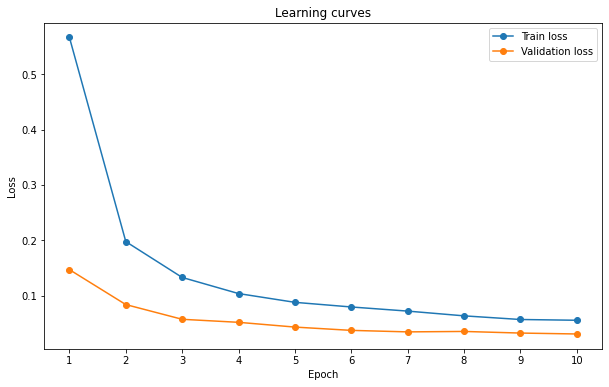
\includegraphics[scale=0.48]{curvas1.png}
        \caption{Curvas de entrenamiento y validación para el modelo Simple CNN. Épocas 1-10.}
        \label{fig:curvas1}
    \end{figure}
    
    Como podemos ver en la Figura \ref{fig:curvas1}, la función de pérdida va decreciendo mucho más en el conjunto de validación que en el conjunto de entrenamiento, por lo que vemos que no hay \emph{overfitting}.
    Es posible que este efecto se deba a la inclusión del \emph{Dropout} en entrenamiento, ya que esto regulariza por la capacidad de ignorar determinadas neuronas durante el entrenamiento. Tampoco se observan 
    problemas de \emph{high-bias}, ya que la pérdida siempre decrece, por lo que podemos ver que el modelo está aprendiendo.

    \begin{table}[H]
        \centering
        \begin{tabular}{l c|l}
        \multicolumn{1}{c}{}             & \cellcolor[HTML]{E3E7EC}Mejor precisión (validación) & \cellcolor[HTML]{E3E7EC} Época con mejor precisión \\ \hline
        \cellcolor[HTML]{E3E7EC}Simple CNN & 98.94\%                                              & \multicolumn{1}{c}{10}   \\ 
        \end{tabular}
        \caption{Mejor precisión con su correspondiente época, obtenida por el modelo.}
        \label{table:resultsprec}
        \end{table}

    La mejor precisión obtenida se alcanza en la última época (ver Tabla \ref{table:resultsprec}), siendo ésta bastante alta. Vista la progresión de los resultados en cada época (ver primer notebook) y las curvas de aprendizaje,
    es muy posible que el modelo siguiera aprendiendo un poco más. Comprobamos esta suposición más tarde, con 10 épocas más. Adjuntamos los resultados
    en la Figura \ref{fig:curvas12}.
    \begin{figure}[H]
        \centering
        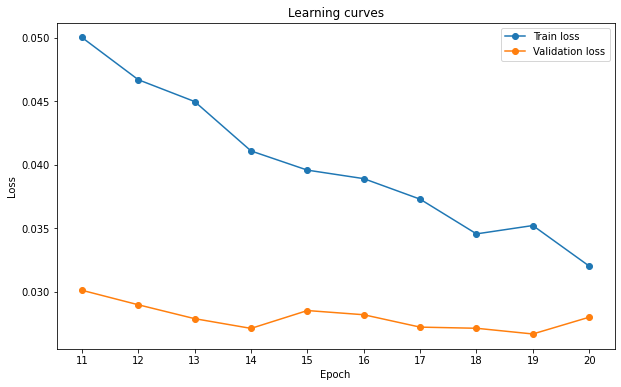
\includegraphics[scale=0.48]{curvas12.png}
        \caption{Curvas de entrenamiento y validación para el modelo Simple CNN. Épocas 11-20.}
        \label{fig:curvas12}
    \end{figure}
    Viendo los resultados en el notebook, conseguimos aumentar la precisión a $99.10\%$ en la época $19$. Observando el comportamiento de la curva y de los resultados, es muy posible que el aprendizaje se hubiera estancado en ese punto.

    \item Incluir la matriz de confusión obtenida. Dada esta matriz de confusión, informe de los 2 casos de confusión entre clases que ocurren con más frecuencia.
    \begin{figure}[H]
        \centering
        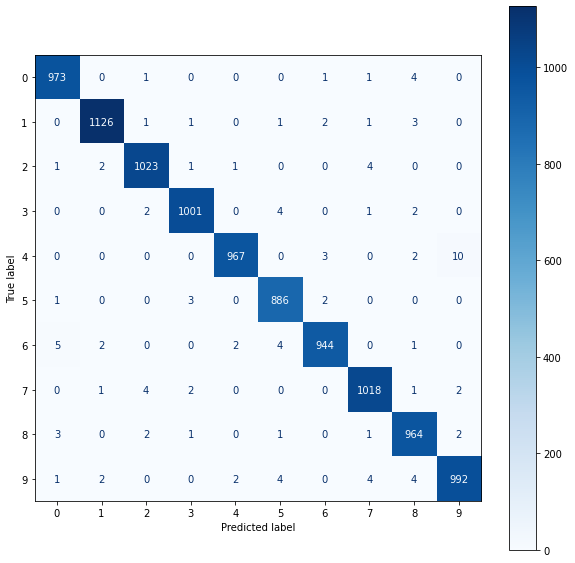
\includegraphics[scale=0.58]{confmatrx1.png}
        \caption{Matriz de confusión de Simple CNN (10 épocas).}
        \label{fig:confmatrx1}
    \end{figure}
    Viendo los resultados, observamos que obtenemos un total de 106 errores de un total de 10000 predicciones. Los errores más comunes se encuentran en el dígito $6$ (tiene muchas confusiones con el $0$, el $5$, etc.), el $4$ (se suele confundir con el $9$), el $5$, incluso el $8$. Podemos ver mejor algunas de estas confusiones en la Figura \ref{fig:errores1}.
    \begin{figure}[H]
        \centering
        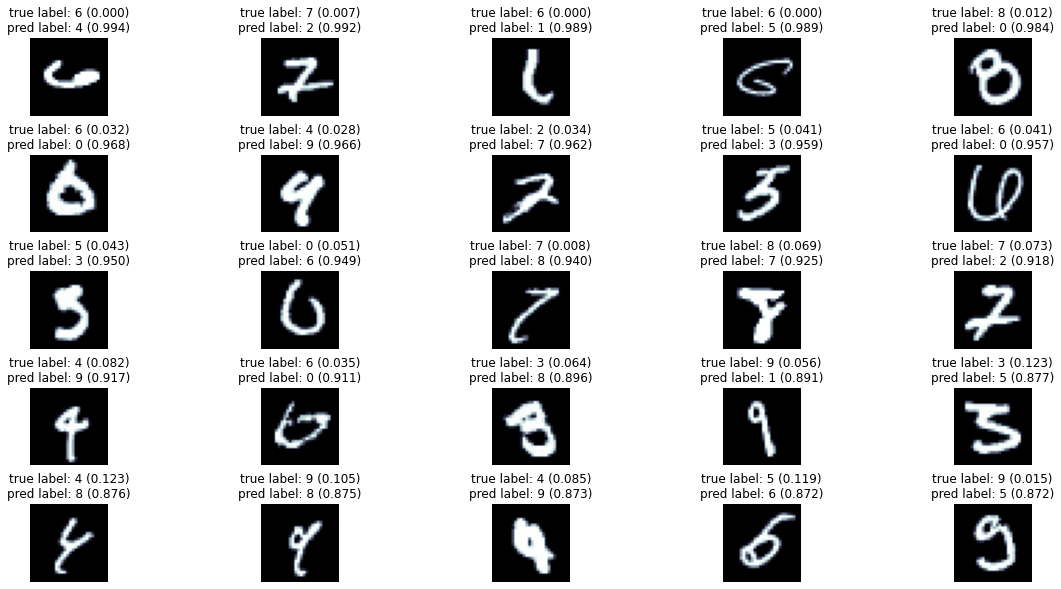
\includegraphics[scale=0.38]{mosterror1.png}
        \caption{Ejemplos de dígitos con más errores en la clasificación.}
        \label{fig:errores1}
    \end{figure}
    
    \item Comente las diferencias entre el gráfico t-SNE de la representación de las capas final e intermedia de la CNN, aplicado a las imágenes del conjunto de validación. Para ello, considere la proximidad y la dispersión entre los clústeres en ambas representaciones, y su relación con la capacidad de realizar una correcta clasificación de las muestras.
    \item Dadas las diferencias entre la representación t-SNE de ambas capas, y dada la arquitectura de la red implementada, identifique en qué capa de la red se extraen las características, y proponga una forma de reducir la complejidad de la red, con una penalización baja en la precisión de la clasificación.
    \end{itemize}

    
\end{document}